\chapter{Extreme Multi-label Learning for Semantic Matching in Product Search}

\textbf{Reference:}~\url{https://arxiv.org/abs/2106.12657}

\textbf{Keywords:} classification, retrieval

\section*{Какую задачу решают авторы?}

Как мы уже неоднократно говорили до этого, использование одного только полнотекстового поиска на данный момент недостаточно для эффективного решения задачи отбора кандидатов для ранжирования.
Популярный способ семантического поиска --- использование DSSM в сочетании с \textit{приближенным поиском ближайших соседей} (ANN) для эффективного отбора кандидатов. \\

Исследователи из Amazon утверждают, что применение даже такой сравнительно неглубокой сети как DSSM, для построения вектора запроса, занимает слишком много времени (не говоря уже об использовании боле сложных архитектур). \\

В данной работе авторы предлагают несколько по иному взглянуть на задачу отбора кандидатов, а именно как на задачу \textit{eXtreme Multi-label Classification (XMC)}. 
То есть по запросу предсказывать какие товары могут быть релеванты (в данном случае, товары и есть классы).
Стоит отметить, что в случае с Amazon'ом речь идет о каталоге размером в $100M$ товаров.  \\

Для эффективного решения данной задачи авторы предлгают подход на основе иерархической линейной модели, который позволяет обрабатывать запросы за логарифмическое от количества товаров время.
Предложенный подход не только позволяет обрабатывать запросы за существенно меньшее время в сравнении с DSSM, но еще и позволяет добиться гораздо большей полноты ($+65\%$).

\section*{Как решают?}

\paragraph{Интуиция} Для начала посмотрим на то как можно решить задачу XMC используя набор \textit{One-vs-Rest (OVR)} линейный классификаторов.
Мы могли бы для каждого товара в каталоге обучить OVR модель, которая по запросу предсказывала бы насколько выбранный товар релевантен для заданного запроса.
Мы можем посчитать такие меры релевантности для всех товаров из каталога и выбрать в качестве результата только те товары, значение релевантности которых больше выбранного порогового значения. \\

Однако, нам бы очень хотелось избежать необходимости вычислять значения релевантности для всех товаров из каталога.
Наверное, самый простой способ ускорить процесс поиска - построить кластеризацию товаров, и считать релевантность не для отдельных товаров, а для целых кластеров.
Представим, что мы сначала выбираем один или несколько кластеров, а затем уже отбираем конкретные товары в рамках отобранных кластеров.
В своей работе авторы развивают эту идею и предлагают использовать \textit{иерархическую кластеризацию} товаров.

\paragraph{Основная идея} Рассмотрим дерево, которое представляет из себя дерево иерархической кластеризации товаров (см. Рисунок~\ref{fig:amazon_tree}).

\begin{wrapfigure}{r}{0.5\textwidth}
    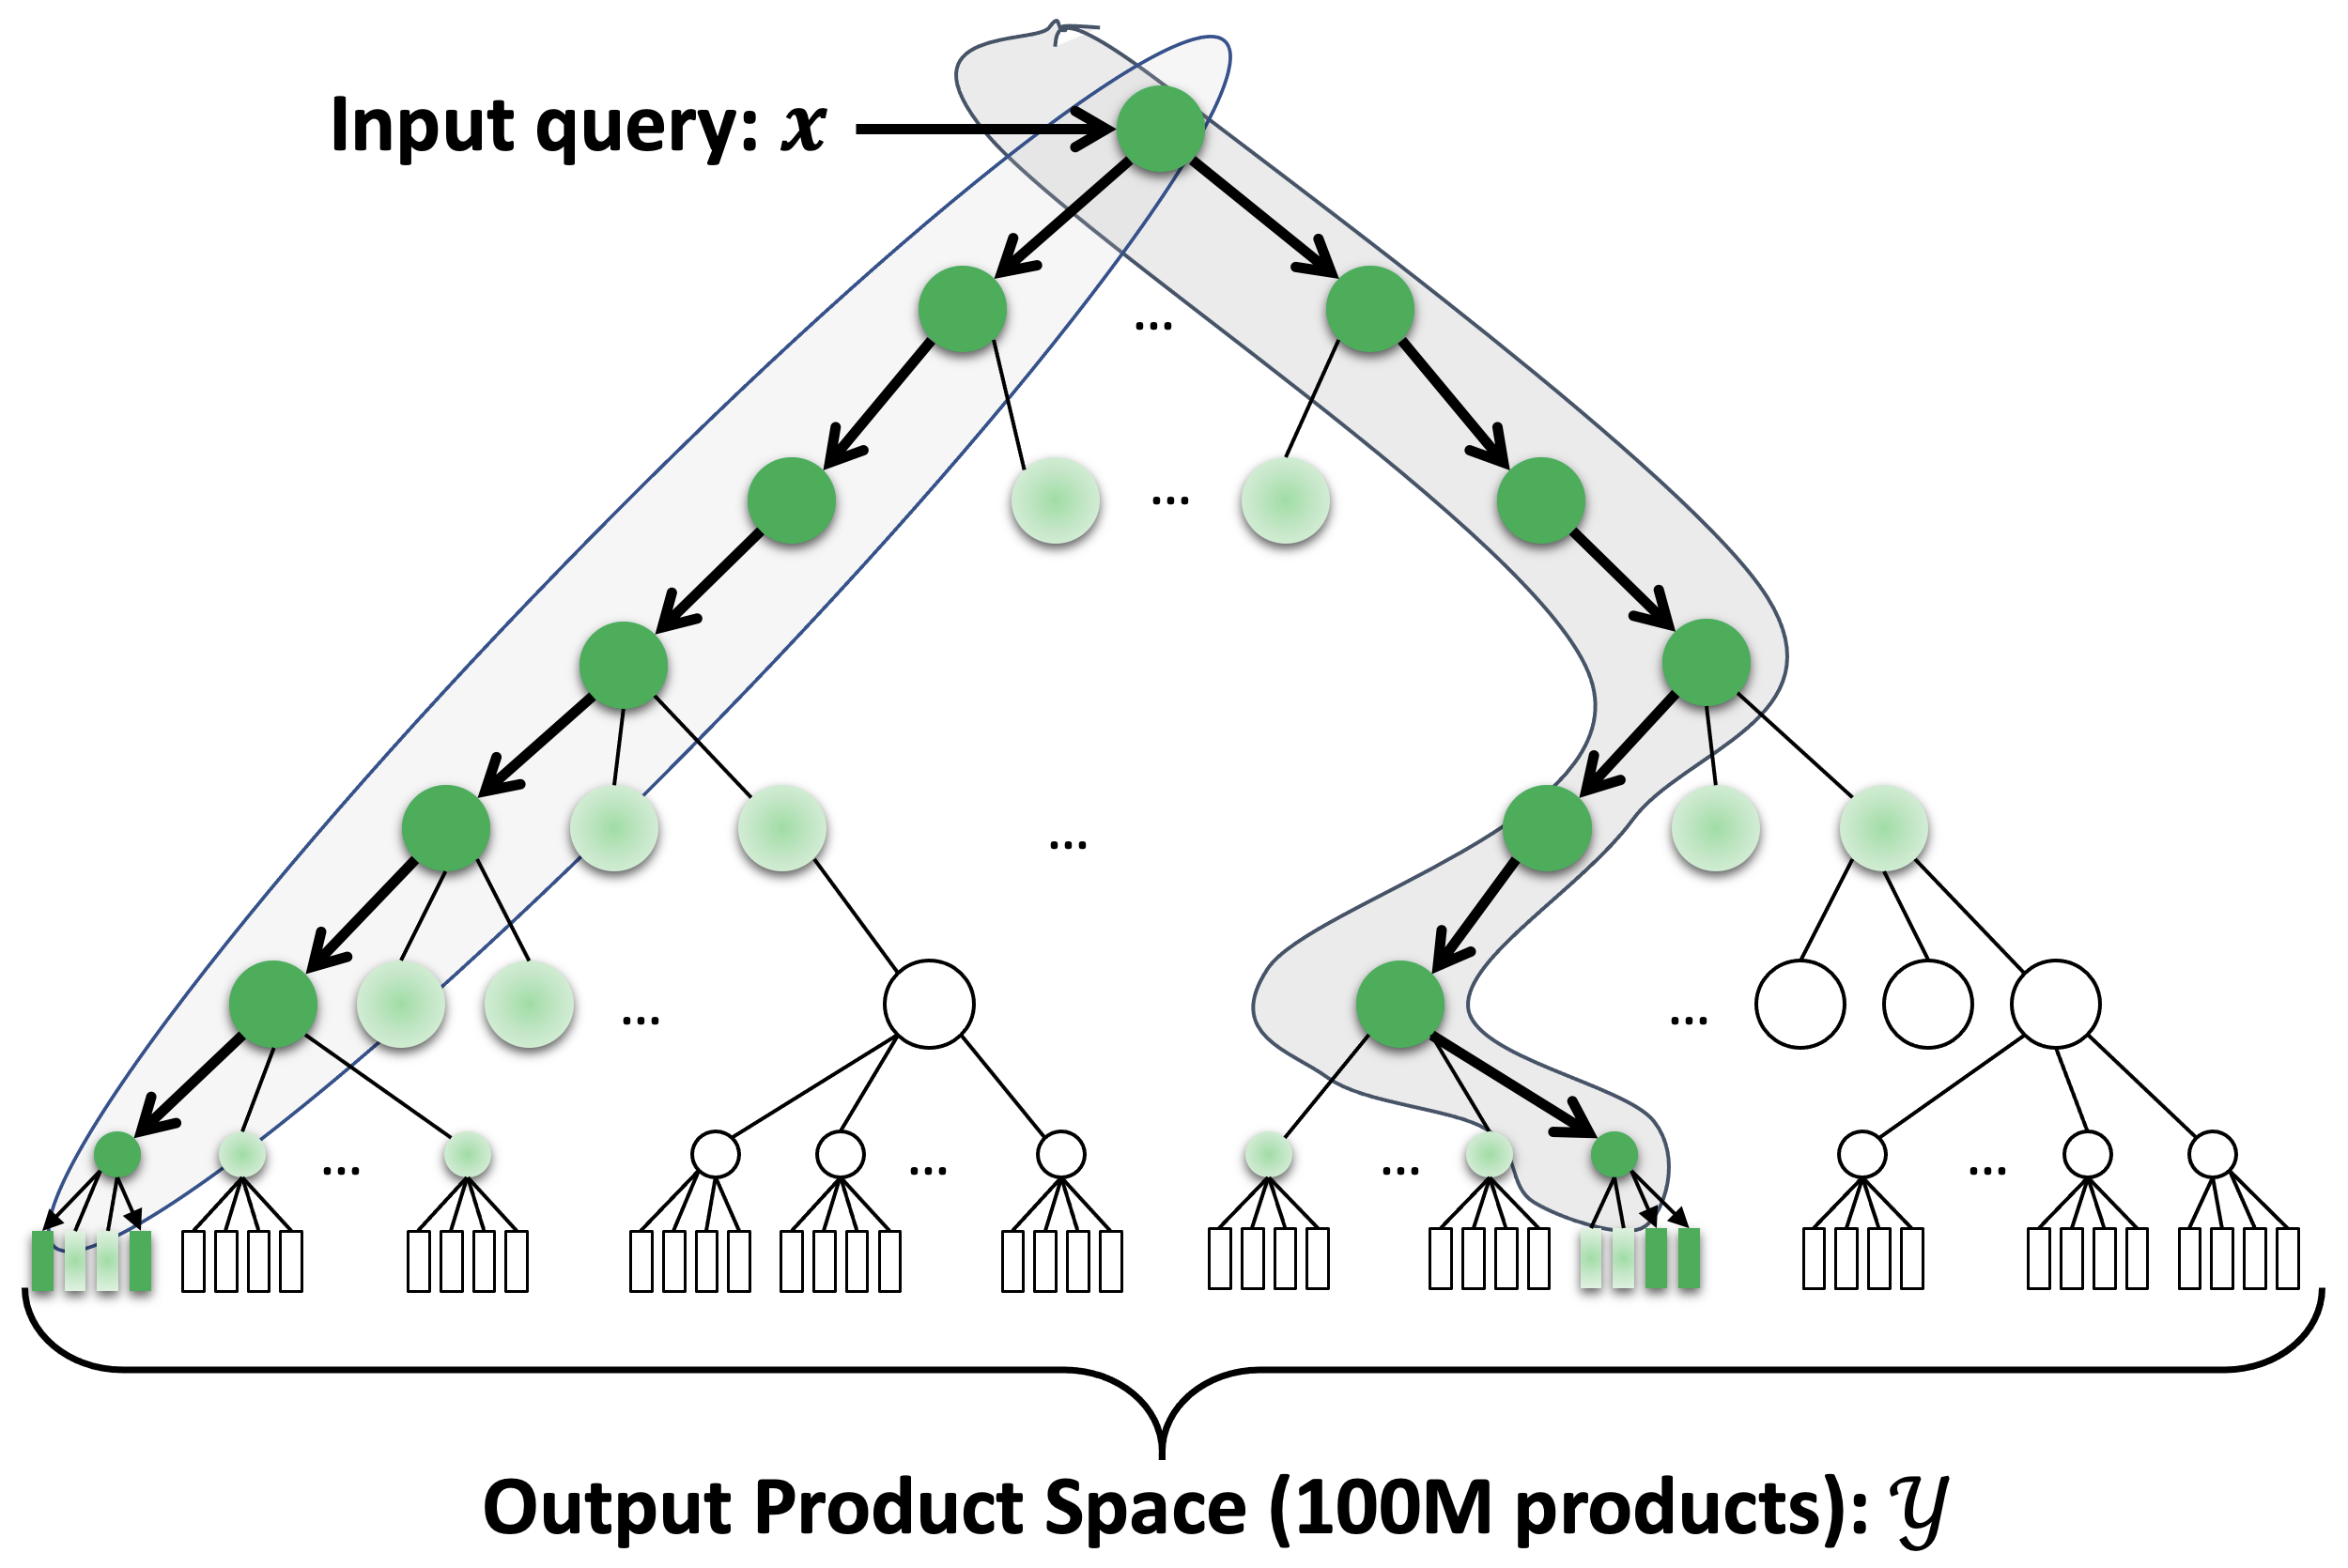
\includegraphics[width=1.0\linewidth]{images/amazon_tree.png}
    \caption{\footnotesize{Illustration of inference using beam search with beam width $b = 2$ to retrieve $4$ relevant products for the given input query $\vecx$}}
    \label{fig:amazon_tree}
\end{wrapfigure}

Листьями данного дерева являются непосредственно товары из каталога, а внутренними узлами - кластеры товаров.
С каждым узлом дерева ассоциирован OVR классификатор, который позволяет оценить релевантность кластера товаров по запросу пользователя. \\

Для того чтобы по запросу эффективно найти множество релевантных товаров, авторы предлагают использовать \textit{Beam search} (см. Рисунок~\ref{fig:amazon_tree}). 
То есть мы будем выполнять спуск по дереву сверху вниз при этом поддерживая множество лучших кандидатов фиксированного размера. 
Для оценки качества кандидатов как раз используются меры релевантности, полученные с помощью классификаторов в узлах деревьев.
Важно отметить, что релевантность конкретного узла (кластера) есть произведение релевантностей всех родительских узлов в дереве на пути к нему. 
Данный способ поиска очень хорошо параллелится, и немного напоминает \textit{Hierarchical softmax}. \\

Теперь подробнее рассмотрим вопросы того как выполнить иерарахическую кластеризацию товарова и как обучить классификаторы в узлах дерева.

\subsection*{Hierarchical Label Tree}

Прежде всего для того чтобы выполнить кластеризацию товаров нужно представить их в векторном виде.
Авторы не настаивают на каком то конкретном способе получения векторных представлений, но сами используют \textit{n-gram TFIDF} представление для товаров на основе их названия и описания. \\

Для построения дерева иерархии используют алгоритм \textit{Spherical B-Means}.

\subsection*{Learning OVR Classifiers}

Ранее мы уже говорили о том, что в каждом узле дерева находится OVR классификатор для оценки релевантности узла (кластера) для данного запроса.
Теперь рассмотрим процедуру обучения классификаторов. 
Прежде всего нужно подготовить данные для обучения. 
Подготовка данных выполняется проходом по дереву снизу вверх.\\

Для начала рассмотрим на каких данных обучаются классифкаторы в листьях дерева, то есть классификаторы для отдельных товаров.
Для конкретного товара множество \textit{положительных} примеров - это множество поисковых запросов при которых был совершен клик по данному товару.
Так как обучается OVR классификатор, то в качестве негативных примеров могут выступать запросы, при которых пользователи кликали на другие товары.
Запросы векторизуются с помощью \textit{n-gram TFIDF}. \\

Теперь рассмотрим то как формируются данные для обучения для внутреннего узла дерева, при условии что уже подготовлены данные для обучения кассификаторов в дочерних узлах.
Фактически в качестве положительных примеров будут выступать все запросы, которые встречаются в качестве положительных примеров в дочерних узлах.
Негативные примеры также как и раньше генерируются случайным образом. \\

Стоит заметить, что после того как готовы данные для обучения, обучение самих моделей можно выполнять независимо друг от друга в параллельном режиме, что позволяет существенно съэкономить время в сравнении, например, со временем обучения DSSM (DSSM обучается примерно в 6 раз медленне).

\subsection*{Results} 

В статье приводят как результаты оффлайн экспериментов, в рамках которых предложенное решение не только позволяет выполнять поиск более эффективно, но еще и с существенно большей полнотой, так и результаты онлайн AB тестов, где авторы так же показывают превосходство нового подсхода в сравнении с DSSM.

\section*{Мое мнение}

Было бы очень интересно узнать как авторы планируют решать задачу холодного старта для товаров, и как часто переобучать модель.